\documentclass{article}

% set font encoding for PDFLaTeX or XeLaTeX
\usepackage{ifxetex}
\ifxetex
  \usepackage{fontspec}
\else
  \usepackage[T1]{fontenc}
  \usepackage[utf8]{inputenc}
  \usepackage{lmodern}
  \usepackage{graphicx}
  \usepackage{float}
\fi

% used in maketitle
\title{
        \begin{center}
        
\includegraphics[width=8cm]{Unison.png}
        \end{center}
        \newline
        Reporte de Actividad 5: Preparando datos con Emacs}
\author{José Burruel}
\date{6 de Marzo del 2018}

% Enable SageTeX to run SageMath code right inside this LaTeX file.
% documentation: http://mirrors.ctan.org/macros/latex/contrib/sagetex/sagetexpackage.pdf
% \usepackage{sagetex}

\begin{document}
\maketitle
\section{Introducción}
En esta sesión de la clase lo que hicimos fue un proceso donde tomabamos un archivo de datos y lo limpiabamos, quitando toda la información basura con la cual no trabajaríamos.

\section{Fundamentos}
La información necesaria para poder realizar esta actividad esta actividad es el manejo del editor de textos \textit{emacs} con el cual realizaríamos la limpieza de los archivos de datos para poder trabajarlos en \textit{Python}.
Otros conceptos que necesitamos para trabajar esta actividad es el concepto de las variables CAPE y PW que necesitamos de los archivos ya mencionados:
\subsection{CAPE}
Energía Potencial Convectiva Disponible (o CAPE, por las siglas del inglés Convective Available Potential Energy) es la energía que tendría una parcela de aire si fuera ascendida verticalmente cierta distancia en la atmósfera.
El CAPE es efectivamente la flotabilidad positiva que tiene una parcela de aire y es un indicador de la inestabilidad atmosférica, lo que significa que si este indicador es alto, se prevee un Tiempo meteorológico severo.
\subsection{PW}
Esto es el Agua Precipitable (PW por sus siglas en ingles) es la cantgidad de vapor de agua contenido en una parcela de aire atmosférico que está en riesgo de precipitar y caer al suelo en forma de gotas.

\section{Procedimiento}
Para empezar, de los archivos utilizados la práctica pasada, en esta ocación tomamos parte del código y lo modificamos para crear un archivo solo con las variables de CAPE y PW junto con la fecha de estas mediciones.
\begin{verbatim}
egrep -v 'PRES|hPa' sondeos.txt | egrep 'H2|CAPE|Precip' > df2017CAPE_PW.csv
\end{verbatim}

De aquí, lo siguiente era limpiar los acrhivos para quitar la información basura, que es todo el texto que nos dice qué es el valor, cuando nosotros nomás necesitamos los valores de estos indicadores.

\subsection{Limpia de los archivos.}
Lo que se hizo para deshacernos de esta información basura fue abrir el documento en \textit{emacs} y realizar una serie de comandos para poder hacer esta limpia.
    \begin{itemize}
        \item \textit{Ctrl + Espacio:} Esto nos deja seleccionar la parte del texto que         se desea borrar.
        \item \textit{Ctrl + W:} Este comando cortaba esa sección, manteniendola en un           Clipboard para su futuro y trabajo con el.
        \item \textit{Esc + <:} Esto te lleva el cursor de texto hasta el inicio de todo         el documento.
        \item \textit{Esc + \%:} Este comando te permite reemplazar todo el texto                 permitido por lo que quieras; te despliega un area de trabajo en la parte de             abajo de \textit{emacs} en el cual te pide que pongas el filtro de la                   información que deseas reemplazar. Presionas \textit{Enter} para confirmar             el archivo y te pide que ingreses por qué texto lo vas a reemplazar; si vuelves         a presionar \textit{Enter} entonces el menú reemplaza lo que escribiste al                 principio por nada, escencialmente borrandolo.
        \item \textit{!:} Al final, confirmas el proceso con un signo de admiración y             vualá!
    \end{itemize}

\subsection{Los dos archivos de distintas horas.}
Los archivos que acabamos de limpiar contienen mediciones hechas a las 00Z y a las 12Z y estas están mezcladas, lo que tenemos que hacer ahora es separarlas en dos archivos, una con solamente las variables 00Z y otra con solo las 12Z.
Esto se hace a travez de un script que contenga:
\begin{verbatim}
egrep '00Z' df2017CAPE_PW.csv | cut -d" " -f 2- > df00Z.csv
\end{verbatim}

\begin{verbatim}
egrep '12Z' df2017CAPE_PW.csv | cut -d" " -f 2- > df12Z.csv
\end{verbatim}

\subsection{Analisis en \textit{Python} con \textit{Pandas} y \textit{Matplotlib}}
Una vez terminada la limpia de los archivos, procedemos a analizar los datos con Python, lo cual nos da una relación entre estas dos variables, cuyas graficas se presentarán a continuación.

\section{Resultados}
Una vez que corrimos el código en \textit{Python} nos dimos cuenta que el archivo 00Z tenía muchas menos mediciones que el archivo de 12Z, lo cual nos mete un error de intrumentación en nuestras mediciones, por las cuales, las gráficas se ven muy... Carecientes de información, sin embargo aquí se presentan.

\subsection{CAPE}
Aquí se presentan las graficas de la columna CAPE de los archivos 00Z y 12Z

\begin{figure}[H]
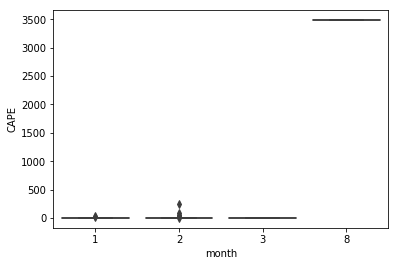
\includegraphics[width=\linewidth]{CAPE00Z.png}
\caption {CAPE del 00Z}
\end{figure}

\begin{figure}[H]
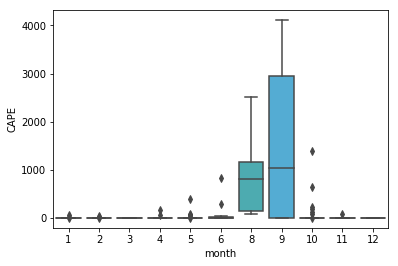
\includegraphics[width=\linewidth]{CAPE12Z.png}
\caption {CAPE del 12Z}
\end{figure}

\subsection{PW}
En esta sección se presentan las gráficas de la columna de Agua Precipitable de ambos archivos.

\begin{figure}[H]
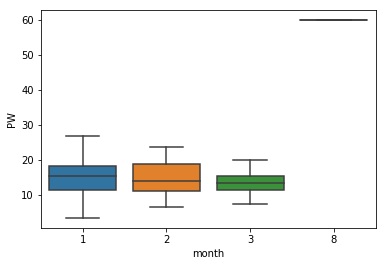
\includegraphics[width=\linewidth]{PW00Z.png}
\caption{Agua precipitable del 00Z}
\end{figure}

\begin{figure}[H]
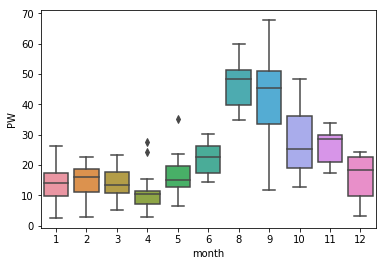
\includegraphics[width=\linewidth]{PW12Z.png}
\caption{Agua precipitable del 12Z}
\end{figure}

\subsection{Interacción entre ambas variables}
Se hicieron dos tipos de gráficas, una es de la relación como tal de ambas variables, y la otra es una regresión para una función que describa esta misma relación. 
Primero, las relaciones como tal: 

\subsubsection{Relación entre las variables.}
Este tipo de gráficas describen la relación encontrada entre CAPE y PW de los archivos leídos. 

\begin{figure}[H]
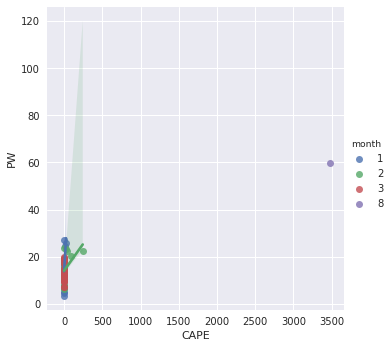
\includegraphics[width=\linewidth]{CAPEvPW_Otros00Z.png}
\caption{Relación entre CAPE y PW del archivo 00Z}
\end{figure}

\begin{figure}[H]
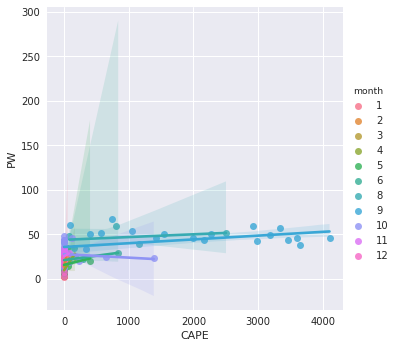
\includegraphics[width=\linewidth]{CAPEvPW_Otros12Z.png}
\caption{Relación entre CAPE y PW del archivo de 12Z, con mayor información.}
\end{figure}

\subsubsection{Regresión entre ambas variables}
Este otro tipo de gráficas describe una función que trata de explicar cómo se relacionan el CAPE y el PW.

\begin{figure}[H]
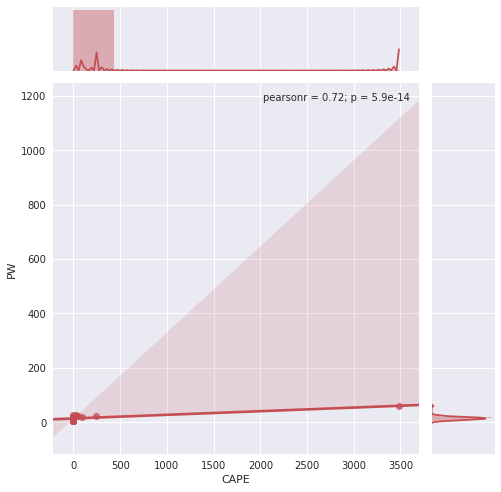
\includegraphics[width=\linewidth]{CAPEvPW_Red00Z.png}
\caption{Regresión de las variables en 00Z}
\end{figure}

\begin{figure}[H]
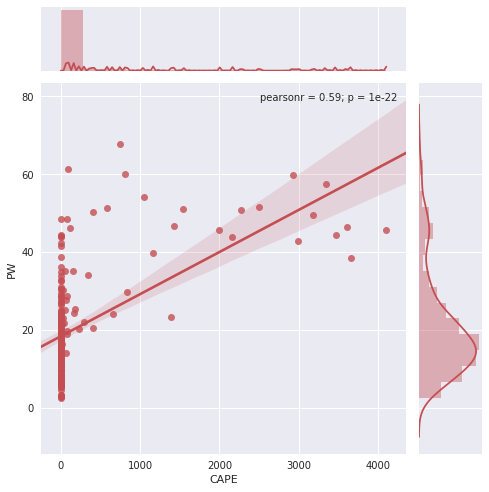
\includegraphics[width=\linewidth]{CAPEvPW_Red12Z.png}
\caption{Regresión de ambas variables en 12Z}
\end{figure}

\section{Conclusiones}
Este aprendizaje de limpia y procesamiento de archivos nos hacen la vida más fácil al querer describir estas relaciones y fenómenos estadísticos a la hora de analizarlos. 
Sin duda, el proceso de archivos en \textit{emacs} nos servirá bastante en un futuro para nuestra carrera profesional.

\newpage

\section{Bibliografía}

\begin{itemize}
\item Curso sobre interpretación de mapas meteorológicos: la CAPE (Convective Available Potencial Energy). (2013, May 27). Visto en 5 de Marzo del 2018

$https://www.tiempo.com/ram/800/curso-sobre-interpretacin-de-mapas-meteorolgicos-el-cape-convective-available-potencial-energy/$

\item Convective Available Potential Energy (CAPE) (Meteorología e hidrología (inglés-español)). Visto en Marzo 5 del 2018

$https://glosarios.servidor-alicante.com/meteorologia-hidrologia_en-es/convective-available-potential-energy-cape$

\item A. Agua precipitable. Visto en 5 de Marzo del 2018

$http://www.aguamarket.com/diccionario/terminos.asp?$

\end{itemize}

\newpage

\section{Apéndice}
\subsection{¿Cómo se te hizo esta actividad? ¿Compleja, Difícil, Sencilla?}
Está bastante sencilla, la verdad. Nos proporciona una herramienta de trabajo de datos antes de su análisis.
\subsection{¿Qué te llamó más la atención?}
La facilidad del procedimiento de limpieza O:
\subsection{¿Qué parte fue la que menos te interesó hacer?}
Ya se la sabe, profe, el reporte.
\subsection{¿Cómo mejorarías esta actividad? ¿Qué le faltó? ¿Qué sobró?}
Está muy completa, la verdad. No se me hace que le falte algo o le sobre nada.
\subsection{¿Hasta este punto, que te parece el uso de Jupyter para programar en Python? }
Está bastante interesante y fácil de utilizar. 
\end{document}
